% COMPILE WITH XELATEX (topleft menu -> Settings -> Compiler)
\documentclass[10pt,a4paper]{article}
\usepackage{preamble}


\title{Speeding Up Galaxy Cluster Evolution Simulations with Physics-Informed Neural Networks}
\author{Pablo Sarró Sánchez, David Richard Harvey}
\date{June 8th, 2026}

\begin{document}

% Title Page excluded from the word count:

%TC:ignore
% TITLE PAGE like the one moodle (that was a Word doc)
% to be included in the main just after \begindocument 
% with \input (simpler) or \include (does clearpage before and after, better for "independent" sections)

\thispagestyle{empty}   % hides the number on the title page (hides footer and header)
\newgeometry{margin=2.5cm, top=3.5cm, bottom=3.5cm}
% blue color in the template word doc : HEX #1F497D
\definecolor{philo_blue}{HTML}{1F497D}

% Top Block ------------------------------------------------------------------
\begin{center}
    {\color{philo_blue}        
        \LARGE \textbf{\textsc{Speeding Up Galaxy Cluster Evolution Simulations with Physics-Informed Neural Networks}}
        
        \vspace{1cm}
        % last name, first name and department of the authors
        {\large\textbf{
            Pablo Sarró Sánchez, CSE
        }}
    }
\end{center}
 
\vfill
% Middle Block ---------------------------------------------------------------
\begin{center}
    %\includegraphics[width=0.4\textwidth]{frog.jpg}
    %\vspace{1cm}
    \large
        Semester Project \nth{1} year master\\[0.6em] 
        Supervised by\\[0.6em]
        {\color{philo_blue}
        \textit{David Richard Harvey, Philosophy of Science}}\\[1.5em]
        Report submitted on June 8th, 2026
\end{center}

\vfill
% Bottom Block ---------------------------------------------------------------
\begin{center}
    \begin{minipage}{\textwidth}
        \centering
        {\large Lausanne, academic year 2025--2026}\\[1.5cm]
        
        % EPFL pdf logo
        
\includegraphics[width=0.2\textwidth]{EPFL_logo.pdf}
    \end{minipage}
\end{center}

\restoregeometry

\setcounter{page}{1}    % restart numbering at 1 for the next page 
%TC:endignore


%\maketitle
% custom title this way:
\makeatletter % treat '@' as a valid letter -> allows access to internal LaTeX macros
\begin{center}
    \Large \textbf{\textsc{\@title}}\\[4pt]
\end{center}
\begin{center}
  {\normalsize \@author \par}
  \vspace{0.2em}
  {\small \@date \par}
\end{center}
\makeatother % restore @ to special character -> hides internal macros

% they want the
% Abstract excluded from the word count:

%TC:ignore
\begin{abstract}
Tracking non-equilibrium primordial chemistry in cosmological simulations is very computationally expensive due to the extreme stiffness of the governing ordinary differential equations. While deep-learning surrogate models offer significant acceleration, they suffer from rapid error accumulation and unphysical drifts during long-term iterative predictions. This work investigates using mass-conserving Physics-Informed Neural Networks (PINNs) to emulate the primordial hydrogen network of the Grackle library. We evaluate two dataset design strategies to address iterative instability: a variance-stratified dataset (Model A) and a phase-space kNN-balanced dataset (Model B). Our results identify two foundational failure modes: Model A develops an ``activity bias'', hallucinating non-existent transitions on stable profiles, whereas Model B suffers from an ``equilibrium bias'' given by temporal data dilution, where static states are overrepresented over high-gradient physical transitions, forcing the network to predict a constant log-increment. To resolve these limitations, we suggest some potential improvements, including a gradient-based filtering with a localised $\delta$ window buffer, a sparse Mixture of Experts architecture, and a Grackle data generation redesign. This work shows the difficulty of constructing training distributions that adequately balance active and equilibrium regimes, a necessary step to develop accurate and rapid surrogate models for galaxy cluster evolution simulations.
\end{abstract}
%TC:endignore


\textbf{Key words:} Cosmological simulations; Stiff ordinary differential equations; Physics-informed neural networks; Surrogate modelling.
\vspace{1.5cm}

\begin{multicols}{2}

\section{Introduction}

Dark matter remains one of the most fundamental open problems in modern astrophysics and cosmology. Although it is inferred to constitute the majority of the matter content in the Universe, its physical nature is still unknown. Understanding what dark matter is, how it behaves, and how it is distributed across cosmic structures is therefore a central goal in contemporary research \cite{taylor2010}.

A key difficulty in studying dark matter arises from the fact that it does not interact with electromagnetic radiation. It is therefore invisible to direct observation and can only be detected through its gravitational influence on visible matter. This makes galaxy clusters especially relevant, as they represent massive gravitationally bound structures, and contain large fractions of dark matter \cite{kravtsov2012formation}.

Despite their importance, observational data of galaxy clusters alone is insufficient to fully characterise their formation and evolution across time, both due to limited resolution and incomplete coverage of parameter space. This motivates the use of predictive models capable of generating realistic galaxy cluster evolutions, which can be then compared with observations. Large amounts of simulations are needed for cosmological inference problems, like parameter estimation or the computation of statistical quantities like covariances, which rely on sampling a wide range of possible physical conditions \cite{schaye2023flamingo, wu2015rhapsody, harvey2025darkskies}.

To achieve this, numerical simulation tools are commonly employed. In particular, hydrodynamical and chemical evolution codes are used to model the coupled evolution of baryonic gas, chemical species, and radiative cooling processes, allowing for realistic modelling of galaxy formation within dark matter halos \cite{kere2009}. A widely used framework is the Grackle chemistry and cooling library \cite{smith2017grackle}.  However, these physical processes are highly non-linear and stiff, which requires implicit integration schemes and adaptive time-stepping approaches. As a result, each simulation becomes computationally expensive, particularly in modern high-resolution codes where millions to billions of resolution elements must be evolved over many timesteps.


% These are computationally expensive due to the stiff, non-linear behaviour of the coupled ordinary differential equations governing the thermal and chemical evolution.


This computational cost motivates the use of machine learning techniques (surrogate models) capable of speeding up such simulations \cite{harvey2024deep}. In this context, neural networks can be trained on simulation outputs to learn the mapping between physical states and their temporal evolution, where once trained, could replace expensive numerical integration with fast function evaluation. However, purely data-driven approaches risk violating fundamental physical constraints, leading to physically inconsistent predictions outside the training distribution \cite{raissi2019physicsinformed}.

Additionally, previous studies have shown that while one-step prediction accuracy can be high, long-term iterative application of learned models can suffer from stability issues, as small errors accumulate over time and lead to diverging trajectories \cite{bourrat2026}.

To address this limitation, Physics-Informed Neural Networks (PINNs) provide a framework in which physical laws are incorporated directly into the learning process through additional constraints in the loss function. This allows the model not only to reproduce simulation outputs, but also to respect the underlying governing equations, improving generalisation and physical consistency \cite{raissi2019physicsinformed}.

In this project, we investigate the use of PINNs to accelerate galaxy cluster evolution simulations by learning the coupled evolution of baryonic gas chemistry and radiative cooling processes as implemented in Grackle. The goal is to develop a surrogate model that preserves physical fidelity while significantly reducing computational cost, enabling more efficient exploration of galaxy cluster dynamics and dark matter properties.

The remainder of this report is structured as follows. Section 2 introduces the physical and numerical formulation of the Grackle solver (Section 2.1) and describes the machine learning methodology used to construct the surrogate model (Section 2.2). Section 3 presents the results of iterative predictions. Section 4 discusses limitations, stability considerations, and perspectives for integration into full cosmological simulations.


\section{Methodology}
\subsection{Chemistry solver : Grackle}

Grackle \cite{smith2017grackle} is a stand-alone chemistry solver that can be integrated with many commonly used cosmological simulation codes like SWIFT \cite{schaller2024swift}. We will aim to create a model that can predict solutions to the non-equilibrium chemistry equations solved by Grackle, thereby accelerating SWIFT's simulations. Grackle deals with a chemical network of up to 12 species by evolving them via chemistry and cooling, but we will use its most simplified version by considering only primordial chemistry species: H, $\mathrm{H}^{+}, \mathrm{He}, \mathrm{He}^{+}, \mathrm{He}^{++}, e^{-}$\footnote{From now on, we write HII instead of $\mathrm{H}^{+}$, and HI instead of H.}. Additionally, we simplified the network further by setting the abundance of all helium species to zero ($n_{\mathrm{He}} = n_{\mathrm{He}^{+}} = n_{\mathrm{He}^{++}} = 0$), which directly implies that the electron number density is the same as the ionised hydrogen density: $n_{\mathrm{e}^{-}} = n_{\mathrm{HII}}$. This simplification serves as an initial baseline to validate our Physics-Informed Neural Network (PINN) architecture before scaling to full multi-species configurations. Furthermore, focusing strictly on the hydrogen network remains physically relevant in specific astrophysical contexts, such as the early stages of cosmic reionisation.

First, Grackle deals with the chemical rate equations, a system of coupled ordinary differential equations describing the rate of change of the species densities. They can be expressed as:

\begin{equation}
\frac{\partial n_{i}}{\partial t}=\sum_{j} \sum_{l} k_{jl}^{(i)} n_{j} n_{l}+\sum_{j} I_{j} n_{j}
\end{equation}

where $n_{i}$ is the number density of species $i$, $k_{jl}^{(i)}$ is the rate coefficient for reactions involving species $j$ and $l$ that act as source or sink terms for species $i$ via collisional processes, while $I_{j}$ corresponds to the radiative rate. Again, we chose to simplify the problem by assuming no radiation, which physically corresponds to an optically thick regime or gas before the epoch of cosmic reionisation, where the ambient ultraviolet background (UVB) radiation field has not yet been established by the first stars and quasars. This means that $I_{j}=0$ for all species $j$.

\begin{center}
    \begin{tabular}{l}
    \hline
    Reactions \\
    \hline
    $\mathrm{H}+e^{-} \rightarrow \mathrm{H}^{+}+e^{-}+e^{-}$ \\
    $\mathrm{H}^{+}+e^{-} \rightarrow \mathrm{H}+\gamma$ \\
    % $\mathrm{He}+e^{-} \rightarrow \mathrm{He}^{+}+e^{-}+e^{-}$ \\
    % $\mathrm{He}^{+}+e^{-} \rightarrow \mathrm{He}+\gamma$ \\
    % $\mathrm{He}^{+}+e^{-} \rightarrow \mathrm{He}^{++}+2 e^{-}$ \\
    % $\mathrm{He}^{++}+e^{-} \rightarrow \mathrm{He}^{+}+\gamma$ \\
    $\mathrm{H}+\mathrm{H} \rightarrow \mathrm{H}^{+}+e^{-}+\mathrm{H}$ \\
    % $\mathrm{H}+\mathrm{He} \rightarrow \mathrm{H}^{+}+e^{-}+\mathrm{He}$ \\
    $\mathrm{H}+\gamma \rightarrow \mathrm{H}^{+}+e^{-}$ \\
    % $\mathrm{He}+\gamma \rightarrow \mathrm{He}^{+}+e^{-}$ \\
    % $\mathrm{He}^{+}+\gamma \rightarrow \mathrm{He}^{++}+e^{-}$ \\
    \hline
    \end{tabular}
    \captionof{table}{List of chemical reactions that impact our scenario, where only $\text{H}, \text{H}^{+}$ and $e^{-}$ are tracked as active chemical species.}
    \label{tab:reacts}
\end{center}

The reaction rates $k_{jl}^{(i)}$ used in Grackle are based on fits to experimental and theoretical data compiled from various literature sources \cite{smith2017grackle}.

In addition, Grackle also evolves the input parameters via heating and cooling processes. This primarily impacts temperature, but it also has a direct effect on the chemical rates, since $k_{jl}^{(i)}$ are dependent on temperature. This is tackled through the internal energy, which relates to the temperature via the expression:

\begin{equation}
e=\frac{k_BT}{(\gamma-1)\mu m_{H}}
\label{eq:e}
\end{equation}


where $e$ is the specific internal energy, $k_B$ is the Boltzmann constant, $T$ the gas temperature, $\gamma$ is the adiabatic index of an ideal gas, $m_{H}$ is the mass of a hydrogen atom and $\mu$ is the mean molecular weight. This parameter $e$ is then evolved by solving the Lagrangian energy equation:


\begin{equation}
\frac{de}{dt}=-\dot{e}_{\text{cool}}+\dot{e}_{\text {heat}}
\label{eq:de/dt}
\end{equation}


where $\dot{e}_{\text {cool}}$ and $\dot{e}_{\text {heat}}$ refer to the cooling and heating processes, respectively, depending on the species densities, temperature and chemical rates. To further simplify our approach, cooling is assumed to be the dominating thermodynamic contribution, and hence heating processes are neglected ($\dot{e}_{\text{heat}} = 0$). This is due to the fact that, given our previous zero-radiation assumption, photoionisation and photoheating are removed, and since there are no external photons from stars to strike the atoms and inject kinetic energy into the plasma, the gas lacks its primary astrophysical heating mechanism.


\subsection{Data generation}

To construct the ground-truth dataset, the Grackle chemistry solver was executed across a wide parameter space, with the state variables ($T, n_{HI}, n_{HII}$) recorded at a constant timestep of 100 years. This specific time interval was chosen as a physically meaningful timestep for interstellar medium simulations, as it remains short enough to resolve the highly stiff, rapid cooling timescales and fast chemical recombination phases characteristic of shocked gas. While Grackle internally computes species evolution using customised, scale-invariant internal units (IU), all tracked outputs were converted and stored in absolute physical units (Kelvin for $T$, and $\text{cm}^{-3}$ for species densities) to simplify the unit conversion through the PINN architecture.

A primary challenge in primordial chemistry modelling is that species densities can achieve very low orders of magnitude, frequently reaching concentrations of $10^{-12} \ \text{cm}^{-3}$. For that reason, we chose to store the ground-truth values with added decimal positions, and the entire training and physics pipeline was done using double-precision 64-bit arithmetic rather than standard single-precision 32-bit operations. This helped prevent catastrophic numerical cancellation and round-off errors close to zero, which would otherwise induce unphysical negative densities or artificial violations of mass conservation (at the expense of a higher computational overhead).

\begin{center}
    \begin{tabular}{llll}
    \hline
    Parameter & Min & Max & Unit \\
    \hline
    $T$ & $2.0$ & $8.0$ & $\log(K)$ \\
    $n_{\text{H}} = n_{\text{HI}} + n_{\text{HII}} $ & $-4.0$ & $2.0$ & $\log\left(\text{cm}^{-3}\right)$ \\
    $x_{\text{HII}} = \frac{n_{\text{HII}}}{n_{\text{H}}}$ & 0.0 & 1.0 & -- \\
    \hline
    \end{tabular}
    \captionof{table}{Sampling ranges for the initial conditions. Values are sampled uniformly in log-space for temperature and density, and in linear space for the ionisation fraction.}
    \label{tab:ICs}
\end{center}

\subsubsection{Initial Random Sampling and Variance Stratification}
\label{sec:dataset1}

With this, we first started creating our dataset by simulating a set of 15,000 independent initial conditions by uniformly sampling the parameter space within the ranges observed in Table \ref{tab:ICs}. Each independent simulation was evolved for a total duration of 2.5 Myr, and given the 100-year output cadence, this trajectory length yields 25,000 data points per file, overall giving a dataset with 375 million individual ground-truth points.

Since cosmic cooling trajectories spend a significant time in slow, near-equilibrium configurations, a naive uniform sampling of this raw data would bias the training distribution toward stationary phases. To prevent the Physics-Informed Neural Network (PINN) from developing a ``spectral bias'' that favours predicting static equilibrium states (basically forcing the model to ``stay still''), a stratification strategy was implemented. Every simulation file was scored by calculating the aggregate log-space variance of its gradients across all physical variables, and based on this metric, we can order the dataset according to the activity of each simulation. With this, we extracted the 800 most dynamic files (high-variance shocks and cooling curves), 250 moderately active files, and 250 low-activity flatlines, splitting them into 700, 150, 150 for training, and 100 of each type for validation. With this, our first dataset contained exactly 1,000 files (25 million points) weighted towards higher activity files to ensure that the model could learn shock behaviours, while the validation set consists of 300 files (7.5 million points) as an unbiased diagnostic suite to test the model's generalisation capabilities across all possible simulation behaviours.

\subsubsection{K-Nearest Neighbours (kNN) Rejection Sampling}
\label{sec:dataset2}

An alternative dataset creation approach was also considered, where now the dataset isn't variance-stratified, but rather kNN-balanced according to the system behaviour. To study the behaviour with respect to the initial conditions, the underlying thermodynamic phase space was systematically mapped. A rigid, uniform grid of 5,625 initial conditions was constructed across $(T_0, n_{H,0}, x_{HII,0})$ as given in Table \ref{tab:GridSampl}, and evolved through the Grackle solver.

\begin{center}
    \begin{tabular}{llll}
    \hline
    Parameter & Min & Max & Step \\
    \hline
    $T$ & $2.0$ & $8.0$ & $0.25$ \\
    $n_{\text{H}} = n_{\text{HI}} + n_{\text{HII}}$ & $-4.0$ & $2.0$ & $0.25$ \\
    $x_{\text{HII}} = \frac{n_{\text{HII}}}{n_{\text{H}}}$ & $10^{-4}$ & $0.9999$ & 9 points \\
    \hline
    \end{tabular}
    \captionof{table}{Grid-sampled ranges to study system behaviour. Ionisation fraction was evaluated at representative discrete points ($10^{-4}, 10^{-2}, 0.1, 0.25, 0.5, 0.75, 0.9, 0.99, 0.9999$).}
    \label{tab:GridSampl}
\end{center}

\begin{figure*}
    \centering
    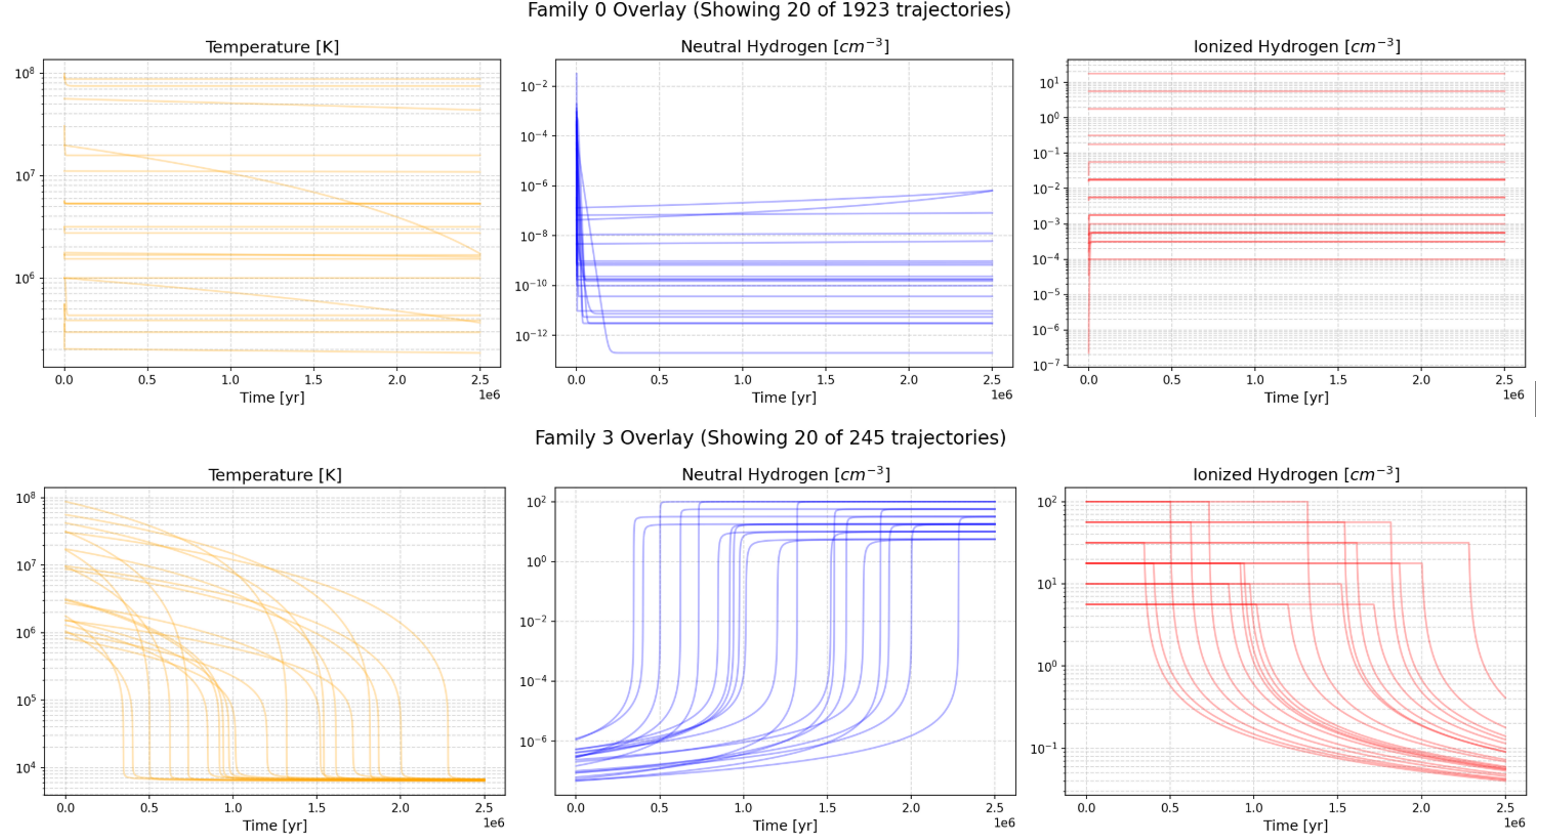
\includegraphics[scale=0.4]{images/Families.png}
    \captionof{figure}{Plot of 20 overlapped trajectories corresponding to the same family. Top: Family 0: hot and ionised equilibrium. Bottom: Family 3: violent recombination and rapid cooling.}
    \label{fig:Families}
\end{figure*}

We generated the trajectories for each of the sampled ICs, after which a K-Means clustering algorithm was applied to classify the phase space into distinct physical regimes. The clustering revealed four fundamental trajectory families: Hot and Ionized equilibrium (Family 0), Low-Density Static Equilibrium (Family 1), High-Density Radiative Cooling (Family 2), and Violent Recombination and Rapid Cooling (Family 3), as shown in Figure \ref{fig:Families}.

This analysis revealed that the thermo-chemical evolution can be grouped in distinct classes of behaviour, depending on the initial temperature and species abundances, where each class shows trajectories with similar cooling histories and ionisation dynamics. However, the differences between classes were often substantial, leading to fundamentally different temporal evolution.

The grid in Figure \ref{fig:IC-grid} exposed a critical aspect: the highly active shock regime (Family 3) occupies less than $5\%$ of the physical phase space. This directly shows that naively generating our dataset by randomly sampling from the set of ICs in Table \ref{tab:ICs} would starve the PINN of active physics data. With this, to ensure the neural network was exposed to a uniform distribution of physical behaviours, this dataset generation technique uses the clustered 5,625-point grid as a ground-truth mapping of the different family behaviours, and a k-Nearest Neighbors ($k=3$) classifier is trained to act as a predictive Oracle.

\begin{figure*}
    \centering
    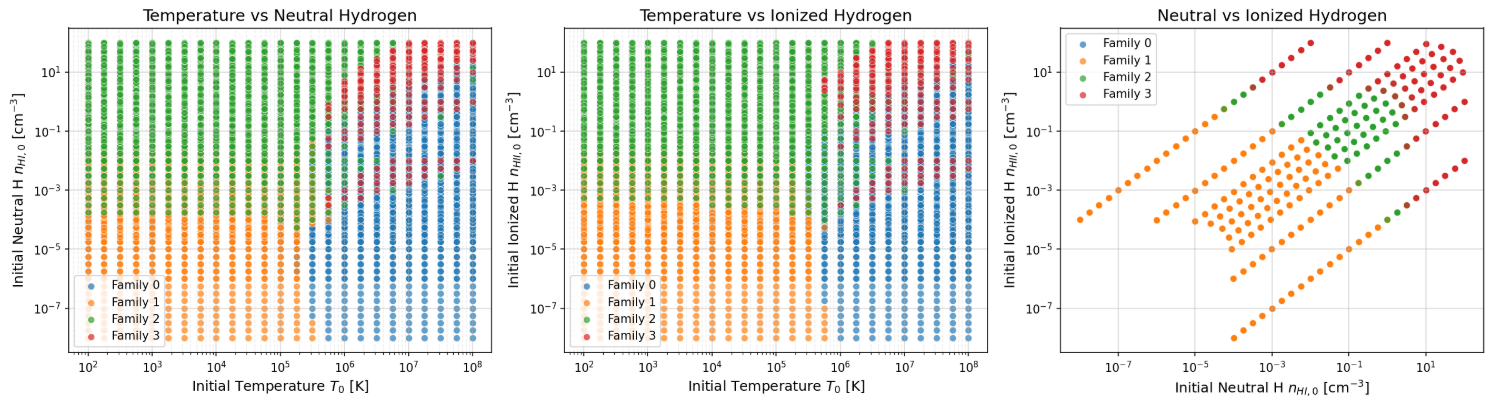
\includegraphics[scale=0.4]{images/IC-grid.png}
    \caption{Thermodynamic phase-space distribution of the grid-sampled initial conditions. Points are colour coded by their assigned trajectory family (Families 0 to 3) using the $\text{kNN}$ classifier oracle.}
    \label{fig:IC-grid}
\end{figure*}

A new stream of initial conditions was generated and passed through the kNN Oracle before simulation, which evaluated the family that it belonged to given its kNN prediction with the ground-truth mapping. This process was repeated until obtaining 250 initial conditions corresponding to each of the 4 families, rejecting a generated initial condition if its family was already represented with 250 other ICs. Hence, the final dataset consists of exactly 1,000 trajectories (250 trajectories per family). From this perfectly stratified distribution, 800 files (200 from each family) were allocated to the training set, while the remaining 200 files (50 from each family) were isolated for validation.

\subsection{Physics-Informed Neural Networks}

A regular neural network attempts to approximate complex non-linear functions \cite{hornik1989} by progressively updating a series of weights and biases, which are organised in a collection of layers containing neurons, followed by a non-linear activation function \cite{goodfellow2016deep}. During training, these parameters are updated by minimising and backpropagating a loss function that measures the difference between the predictions and the true outputs.

Neural networks are still widely used in many different fields of science. However, as purely data-driven models, they act as statistical black boxes which can easily produce physically meaningless predictions, like violating conservation laws or generating negative mass densities.

PINNs solve this limitation by adding the possibility of including the governing physical laws directly into the loss function as regularisation terms. These physics losses constrain the optimisation landscape, forcing the network to search exclusively in a physically meaningful parameter space, which naturally provides consistent and realistic solutions.

\subsubsection{Architecture and Structure}

The core architecture of the PINN consists of a deep, fully connected network, with 12 hidden layers and each layer containing 512 neurons. It uses the hyperbolic tangent ($\tanh$) activation function across all hidden layers rather than the standard Rectified Linear Unit (ReLU). This is done to have more stable gradients throughout the entire phase space, which is especially important in our problem, where the parameter space spans across wide orders of magnitude, and quick temperature and species variations (shocks) are usual during our type of simulations.

The neural network takes a 3-dimensional input vector describing the state of a particle :

\begin{equation*}
\mathbf{x}=\left[\log(T^{(t)}), \log(n_{\text{HI}}^{(t)}), \log(n_{\text{HII}}^{(t)})\right]
\end{equation*}

with $T$ the temperature in Kelvin, and $n_{\text{HI}}, n_{\text{HII}}$ the number density of neutral and ionised hydrogen in $\text{cm}^{-3}$, respectively. In the previous work \cite{bourrat2026}, the input vector included $dt$, but here we assumed a constant $dt$ of 100 years throughout the whole simulation, hence now being an unnecessary parameter to feed to the model.

For better numerical stability, and also motivated by previous work \cite{bourrat2026}, we chose to predict the log-increments of each parameter, rather than its absolute next value. In this way, the output vector of our PINN is given by:

\begin{equation*}
\mathbf{y}=\left[\log\left(\frac{T^{(t+dt)}}{T^{(t)}}\right), \log\left(\frac{n_{\mathrm{HI}}^{(t+dt)}}{n_{\mathrm{HI}}^{(t)}}\right), \log\left(\frac{n_{\mathrm{HII}}^{(t+dt)}}{n_{\mathrm{HII}}^{(t)}}\right)\right]
\end{equation*}

Finally, rather than keeping the learning rate constant, we considered a scheduler that allows it to vary throughout the training phase. This allows the PINN to explore the loss landscape quickly at the beginning of the training phase, and progressively slow down by fine-tuning the weights and biases during later stages. This scheduler starts at an initial value of $10^{-4}$, which halves with a patience of 30 epochs, down to a minimum value of $10^{-6}$.


\subsubsection{Physics and Data Loss Functions}

As we discussed, for PINNs to be helpful, we need to train it using a loss that balances ground-truth data accuracy and known physical principles. This splits the total loss into two primary categories: a data loss, which penalises deviation from the Grackle-generated training samples, and a set of physics losses, which penalise violations of the underlying differential equations and conservation laws governing the system.

The data loss was initially computed via a standard Mean Squared Error (MSE). However, this formulation proved unsuccessful when capturing the exact timing and magnitude of sharp thermal and chemical shocks. As these represent a tiny fraction of the total temporal data points compared to the abundant equilibrium phases, a standard MSE naturally favours optimising the flatlines while ignoring the shocks. In this way, to force the network to understand and learn these critical phases, a customised weighted data loss was implemented:

\begin{equation*}
\mathcal{L}_{\text{data}} = \mathbb{E}\left[(1 + \text{20}|\mathbf{y}|)(\hat{\mathbf{y}} - \mathbf{y})^2\right]
\end{equation*}

Here, the scaling term ($1+20|\mathbf{y}|)$ scales linearly with the magnitude of the true log-increment vector $\mathbf{y}$. In this way, during sharp cooling or ionization bursts where the rate of change is large ($|\mathbf{y}| \gg 0$), the multiplier highly penalises prediction errors. Conversely, in near-equilibrium zones where changes are minimal ($|\mathbf{y}| \approx 0$), the multiplier goes to 1, going back to a standard MSE.

On the other hand, the PINN must also account for physics losses derived from the governing thermodynamic and chemical rate equations to constrain the network's parameters to a physically realistic domain. Ideally, this requires introducing distinct regularisation penalties that enforce the expected continuous derivatives $dT/dt$ and $dn_i/dt$ according to primordial gas dynamics.

For the thermal evolution, we analyse the gas energy equations. We choose to formulate the loss using the volumetric internal energy $u = e\cdot\rho = e\mu m_H n_{\text{tot}}$ (expressed in units of $\text{erg cm}^{-3}$) rather than the specific internal energy $e$ (expressed in $\text{erg g}^{-1}$). Under this framework, the relationship between thermal energy density and temperature simplifies to:

\begin{equation}
u = \frac{k_B T n_{\text{tot}}}{\gamma - 1} = \frac{3}{2} k_B T n_{\text{tot}}
\label{eq:u}
\end{equation}

where $\gamma = 5/3$ is the adiabatic index for a monoatomic gas, and $n_{\text{tot}} = n_{\mathrm{HI}} + n_{\mathrm{HII}} + n_{\mathrm{e}^{-}}$ is the total number density of free particles. Rewriting the Lagrangian energy equation by multiplying both sides of \ref{eq:e} by $\rho$ and approximating the continuous time derivative with a forward discrete difference gives:

\[
-\dot{e}_{\text{cool}} = \frac{u^{(t+dt)} - u^{(t)}}{dt}
\]

where $\dot{e}_{\text{cool}}$ now represents the volumetric cooling rate ($\text{erg cm}^{-3}\text{ s}^{-1}$), and is given by the sum of four radiative contributions: collisional ionisation, collisional excitation, recombination cooling and Bremsstrahlung. This motivates the following physical loss:

\[
\mathcal{L}_{\text{physics, } u} = \mathbb{E}\left[\left(\frac{u^{(t+dt)} - u^{(t)}}{dt} + \dot{e}_{\text{cool}} \right)^2\right]
\]

However, although plots confirmed that this discrete derivative was continuous enough to properly approximate $\dot{e}_{\text{cool}}$ and track the cooling curve well, using it in the loss function led to a significant training instability. This was probably caused by tiny numerical deviations, trying to have the PINN learn through a discrete temporal difference and at the same time a highly non-linear and stiff cooling rate. To resolve this, an alternative formulation was derived by fully differentiating both sides of equation \ref{eq:u}, to solve explicitly for the temperature derivative. Isolating for $dT/dt$ gives:

\[
\frac{dT}{dt} = -\frac{2}{3k_B n_{\text{tot}}}\dot{e}_{\text{cool}} - \frac{T}{n_{\text{tot}}} \frac{dn_{\text{tot}}}{dt}
\]

Which introduces the loss below:

\[
\mathcal{L}_{\text{physics, } T} = \mathbb{E}\left[\left(\frac{dT}{dt} + \frac{2\dot{e}_{\text{cool}}}{3k_B n_{\text{tot}}} + \frac{T}{n_{\text{tot}}}\frac{dn_{\text{tot}}}{dt}\right)^2\right]
\]

However, this expression gave poor convergence as well. Not only do we suffer from the same problem as before, but additionally, now the equation depends directly on the total particle number density derivative $dn_{\text{tot}}/dt$, which is computed from the species rate networks. Consequently, any minor error in the chemical network's predictions propagates directly into the thermal loss, causing unstable gradients during training. Besides, evaluating terms scaled by $1/(k_B n_{\text{tot}})$ again introduces severe numerical instability during backpropagation, as both Boltzmann's constant ($k_B \approx 1.38 \times 10^{-16} \ \text{erg K}^{-1}$) and the trace densities are very close to zero. Due to these accumulated numerical scaling issues and the resulting degradation in training performance, the explicit temperature physics loss was omitted from the final PINN architecture.

Then, for the chemical species, we initially thought about integrating the chemical rate equations directly into the loss function. However, when comparing the time derivatives ($dn_i/dt$) against the computed right-hand side reaction terms ($\sum k_{jl}^{(i)}n_jn_l$) extracted from Grackle, the latter showed a large numerical instability. The calculated reaction rates failed to match the true derivatives, showing many erratic numerical jumps during the whole simulation time before the temperature and species shocks. This breakdown is likely due to the rapidly changing nature of the chemical rate equations, since the reaction rate coefficients $k_{jl}^{(i)}$ are defined in units of $\text{s}^{-1}$, whereas the discrete simulation timestep spans $100\text{ years}$ ($\approx 3.15 \times 10^9\text{ s}$). Hence, even after evaluating all possible combinations of the four primary chemical rates involved, the timescale difference prevented the species derivatives from aligning with the chemical rates.

Alternatively, we considered the mass conservation principle. For a pure hydrogen plasma, the total hydrogen number density must remain constant across all timesteps: $n_{\text{H}}^{(0)} = n_{\mathrm{HI}}^{(t)} + n_{\mathrm{HII}}^{(t)}, \ \forall t$. Initially, a standard MSE loss was applied to minimise the residual between the initial total density and the sum of the predicted species at time $t$:

\[
\mathcal{L}_{\text{mass}} = \mathbb{E}\left[\left(n_{\text{H}}^{(0)} - \left(n_{\mathrm{HI}}^{(t)} + n_{\mathrm{HII}}^{(t)}\right)\right)^2\right]
\]

However, because the absolute number densities can drop to very low orders of magnitude, a standard MSE didn't prove successful and tended to ignore conservation losses, especially for low-density cases. For example, an error between $10^{-7}$ and $10^{-6}$ yields a negligible absolute penalty compared to an error between $1$ and $10$, even though there is the same error factor in both cases. To resolve this scale dependence, we implemented a log-space MSE loss:

\[
\mathcal{L}_{\text{mass}} = \mathbb{E}\left[ \left( \log(n_{\text{H}}^{(0)}) - \log(n_{\mathrm{HI}}^{(t)} + n_{\mathrm{HII}}^{(t)}) \right)^2 \right]
\]

This formulation normalises the penalty across all scales, punishing multiplicative errors in the same way across any order of magnitude. This approach proved to be highly stable and was chosen as the definitive physics loss component for the architecture.

To balance the considered loss functions, PINNs couple them via a weight factor on the physics loss that acts as a regulariser on the total loss, via the following formulation:

\[
\mathcal{L}_{\text{total}} = \mathcal{L}_{\text{data}} + \lambda_{\text{phys}}\mathcal{L}_{\text{mass}},
\]

where the scaling factor $\lambda_{\text{phys}}$ must be carefully chosen so that the magnitude of the physics penalty is comparable to the data loss. Otherwise, if $\lambda_{\text{phys}}$ is too small, the network ignores the physical constraints and overfits the training samples; but if it is too large, the physical constraints overpower the optimisation gradient, leading to significant underfitting.

We evaluated two different approaches for this $\lambda_{\text{phys}}$ adjustment: keeping it constant along the training against linearly scaling it from zero up to its maximum calibrated value over the training, which is a common method for what we call \textit{loss balancing}. Our experiments showed that the latter slightly outperformed the constant weighting strategy. By avoiding the strict enforcement of mass conservation during the initial epochs, the PINN is allowed to freely explore the parameter space and understand the global features of the thermo-chemical evolution without any restrictions. Once an initial baseline is established, the progressive activation of the physics penalty helps to refine the network's representations, refining the weights and guiding them to converge to a physically valid solution while keeping the initial information on the evolution behaviour.

\vspace{3mm}



\section{Results}

The initial objective of this work was to train a single Physics-Informed Neural Network capable of reproducing the thermo-chemical evolution generated by Grackle across the full range of sampled initial conditions described in Table \ref{tab:ICs}. However, as we saw, this contains trajectories that show diverse behaviours depending on the initial conditions, including rapid cooling phases, ionisation transitions and near-equilibrium configurations. To obtain a model capable of generalising to any type of system behaviour, we now evaluate the impact of the two different dataset creation approaches mentioned before. Model A was trained on the initial variance-stratified dataset, and Model B was trained on the kNN-balanced dataset. These correspond to the approaches explained in Sections \ref{sec:dataset1} and \ref{sec:dataset2}, respectively.

\subsection{Model A: Variance-Stratified}

The initial dataset creation approach assumed that weighting the dataset towards high-variance trajectories would force the network to learn the stiff cooling equations. While Model A successfully captured the rapid temperature and species drops typical in Family 3 trajectories, it struggled to generalise across all evolutionary regimes simultaneously, as shown in Figure \ref{fig:modelA-preds}, showing poor performance on long equilibrium trajectories.

\begin{figure*}
    \centering
    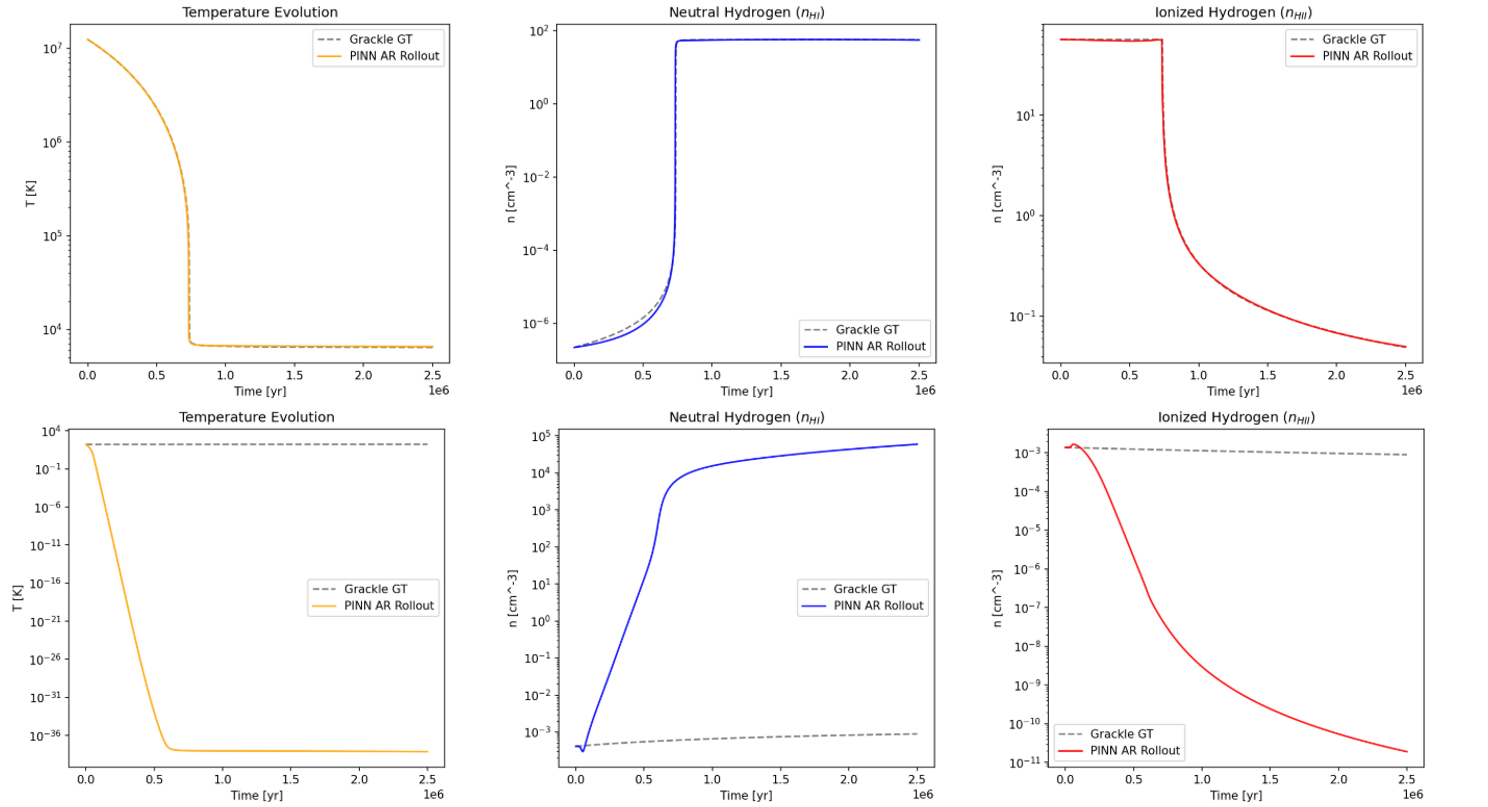
\includegraphics[scale=0.4]{images/modelA-preds.png}
    \caption{Iterative predictions for model A on two different trajectory types. Top: Family 3 trajectory, showing good performance. Bottom: Family 1 trajectory, hallucinating inexistent rapid cooling and recombination rates that aren't there.}
    \label{fig:modelA-preds}
\end{figure*}

Since this approach heavily oversampled active trajectories to capture the ``hard-to-learn'' kinetics, the vast majority of the optimiser's gradient updates were biased towards shock scenarios, or Family 3 trajectories. Consequently, the network failed to learn the trivial low and moderate trajectories which correspond to more steady states. Instead of recognising that flat input conditions should yield zero functional change over time, Model A learned a biased mapping that associates the passage of time with active cooling.

As a result, although performing well for Family 3 trajectories, as shown in Figures \ref{fig:GoodPreds-ModelA} and \ref{fig:GoodPreds2-ModelA}, when presented with stable initial conditions from Family 0, 1, or 2, Model A failed to hold the equilibrium states, instead injecting unphysical transitions into the trajectories, as seen in Figures \ref{fig:fam0-modelA}, \ref{fig:fam1-modelA} and \ref{fig:fam2-modelA}.


\subsection{Model B: kNN-Balanced}
Contrary to what was expected, training Model B on the perfectly balanced dataset (exactly 250 files per family) gave physically inaccurate predictions. Despite successfully resolving the initial condition bias using the kNN oracle, autoregressive rollouts of the trained PINN revealed a catastrophic failure to capture the stiff cooling shocks and recombination transitions for every family.

\begin{figure*}
    \centering
    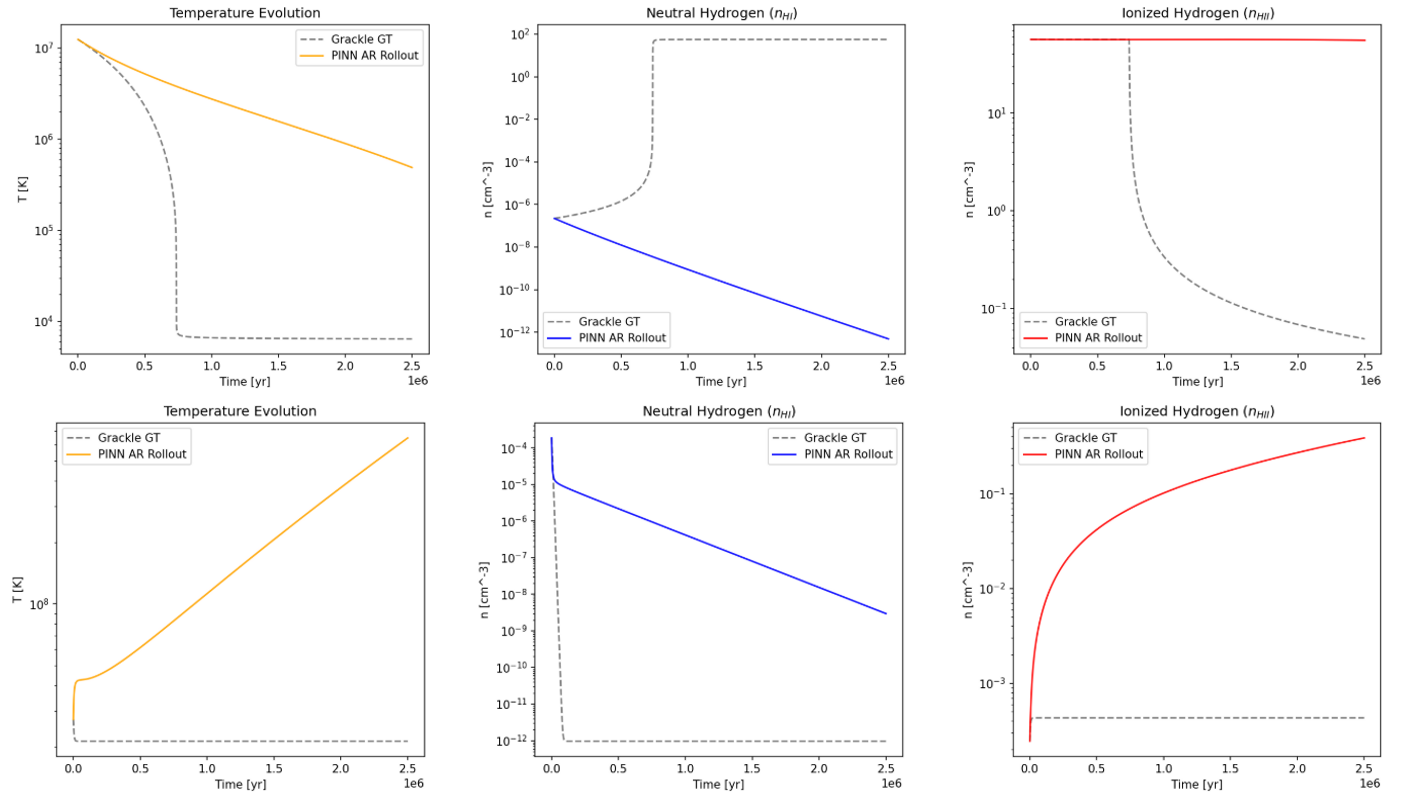
\includegraphics[scale=0.4]{images/modelB-preds.png}
    \caption{Iterative predictions for model B on two different trajectory types. Top: Family 3 trajectory. Bottom: Family 0 trajectory. In both, there is a clear underfitting taking place.}
    \label{fig:modelB-preds}
\end{figure*}

As illustrated in Figure \ref{fig:modelB-preds} (top row), when evaluated on an active Family 3 trajectory, the true Grackle profile undergoes a sharp, highly localised thermal and chemical transition at approximately $0.75$ Myr. Model B entirely fails to resolve this non-linear cliff, and instead produces a perfectly straight, diagonal line in log-space, corresponding to a constant downward drift. Similarly, on a static equilibrium profile (Figure \ref{fig:modelB-preds}), the network shows a steady, unphysical log-linear drift in the output variables.

The cause of these failures is the severe temporal imbalance. Although Model B successfully balanced the dataset across phase-space initial conditions, the data remained temporally uniform. The Grackle simulations contain data at constant integration timesteps of $dt = 100$ yr, resulting in 25,000 points per trajectory. However, due to the extreme stiffness of the primordial chemistry, the highly active non-linear transitions occur in very few steps. The remaining $>99.9\%$ of the temporal domain consists of almost-static equilibrium states where the true physical gradient is close to zero. In the same way, non-active trajectories also contribute to the dataset flatness, since they remain stationary for most of their entire duration, injecting additional flatness into the training dataset. Consequently, the PINN becomes mathematically dominated by this equilibrium state, and so predicting a constant (near-zero) increment state across the entire temporal domain gives a globally minimal (but physically incorrect) data loss ($\mathcal{L}_{data}$). The temperature and species density shocks are so uncommon that they are smoothed out by the huge volume of static data, forcing the network to converge on a ``lazy'' constant value in log-space, which gives rise to these flat lines in linear space.


\section{Discussion: Future Steps}

The structural failures observed in Models A and B demonstrate that optimising PINNs for stiff astrochemical kinetics requires a fundamental shift away from uniform temporal data structures. To overcome the coupled issues of phase-space bias and temporal gradient dilution, two distinct methodological workflows have been designed and are proposed as immediate future steps.

\subsection{Equilibrium Filter}

The failure of the uniform training strategies comes from the huge density of static equilibrium data across the time domain. Because the raw Grackle ground truth data use a fixed timestep of $dt = 100$ yr over a total timeline of $2.5$ Myr, every single trajectory contains exactly 25,000 data points. However, due to the extreme stiffness of primordial cooling, non-linear chemical shocks are compressed into less than $10$ integration steps. Hence, more than $99.9\%$ of the dataset consists of near-equilibrium phases, where the input parameters barely change from $t$ to $t+dt$. This means that log-increments are predominantly zero throughout the whole Grackle file, which biases the PINN to predict a constant near-zero value. However, when performing inference over large timesteps, the smallest error between the true log-increment and the predicted value accumulates, which causes the predictions to be way off the true linear values.

To decouple the system from this equilibrium bias, a gradient-based filtering is proposed as an immediate future step to balance the dataset flatness. This preprocessing approach computes the rate of change across the time-series and enforces a log-gradient threshold:

\[
\left|\log\left(\frac{T^{(t+dt)}}{T^{(t)}}\right) \right| > \epsilon
\]

where $\epsilon$ represents a tunable sensitivity threshold (e.g. $10^{-5}$), such that data points falling below this threshold are removed from the dataset. However, to avoid removing all flatness from the dataset, an explicit window of $\pm \delta$ (e.g. $10$) integration steps around every detected transition is kept in the dataset to also include flat information and allow the PINN to learn about this flatness. Initial implementation of this protocol shows a massive $82\%$ reduction in total data volume, collapsing the training data from around 25 million points down to $\sim$3.6 million points. This downsampling eliminates the equilibrium bias by increasing the density of high-variance, active chemical kinetics in every training batch.

\subsection{Mixture of Experts}

While the temporal filter significantly improves the ratio of active-to-static data, fine-tuning the exact threshold $\epsilon$ and window buffer $\delta$ to perfectly balance active and equilibrium dynamics globally is not trivial. In fact, this active-equilibrium balance is hard to achieve as it has also been seen for models A and B, both of which tried to address this same problem without success.

To bypass this difficulty, an alternative approach is proposed: leverage the pre-identified thermodynamic families to transition from a single global network trying to predict all of them simultaneously to a \textit{Mixture of Experts} (MoE). Rather than forcing one set of neural network weights to resolve diverse system behaviours, the phase space is explicitly partitioned, as given by Figure \ref{fig:IC-grid}. Under this framework, independent, specialised PINN ``experts'' are trained in complete isolation, each dedicated exclusively to a single trajectory family (e.g. training a model solely on Family 3 trajectories). With this, each of them can focus on learning the true underlying pattern and behaviour of its given family, so that, during inference, a trainable gating network determines the sparse combination of these experts to use for each initial thermodynamic state \cite{shazeer2017outrageously}. Ideally, this could provide accurate predictions across both highly active shocks and long-term equilibrium flatlines.

\subsection{Time-Adaptive Data Generation}

While the previous strategies address the problems identified in this work, this last approach addresses their root cause directly during dataset construction. A more robust solution lies in re-engineering the Grackle ground-truth data generation itself by abandoning the constant output of $dt = 100$ yr and instead having our dataset evolve through Grackle's internal adaptive timestep. In this way, the dataset would naturally contain more samples during periods of rapid thermo-chemical evolution, while reducing the large number of nearly redundant equilibrium states present in the current formulation.

The main drawback of this approach is that the timestep $dt$ would no longer be constant and hence would need to be given explicitly as an additional network input. The surrogate model would then be required to learn the system evolution as a function of both the current physical state and the elapsed timestep, increasing the complexity of the learning task. However, this added complexity may be counterbalanced by the benefits of constructing a training dataset that is more closely aligned with the underlying physics. By concentrating samples around periods of rapid thermo-chemical evolution and decreasing the amount of almost-equilibrium states, this strategy could improve data efficiency, thus reducing the need for detailed trajectory classification or heavily weighted loss functions. Overall, this could improve the model's ability to generalise across the diverse trajectory behaviours found in Grackle simulations.

\section{Conclusions}

This project systematically investigated the application of Physics-Informed Neural Networks (PINNs) as fast, high-fidelity surrogate emulators for the non-equilibrium primordial chemistry and radiative cooling equations implemented in the Grackle library. We built directly on top of the exploratory baseline work done by Bourrat \cite{bourrat2026}, which demonstrated that feedforward architectures can recover single-step gas behaviour with high precision. In this way, this work addressed the challenge of long-term iterative stability during multi-step iterative predictions, where several important advancements were introduced to improve the model's capabilities with respect to prior implementations.

First, a deeper network of 12 hidden layers and 512 neurons per layer was used to avoid underfitting, at the expense of increased training computation cost. Then, a constant timestep of $dt = 100$ was used throughout the ground truth data, reducing unnecessary input dimensionality. Additionally, an increased floating point arithmetic was used to improve numerical stability during low-order chemical species density. Finally, rather than relying exclusively on post-prediction renormalisation to correct for conservation errors \cite{bourrat2026}, this work directly embedded a log-space mass conservation penalty ($\mathcal{L}_{\text{mass}}$) into the loss function during backpropagation, which was gradually imposed throughout training with a linear loss-balancing schedule ($\lambda_{\text{phys}}$).

Through a structured sequence of optimisations, we analysed two primary approaches that allowed us to study the thermochemical problem at hand. First, Model A featured an increased sampling of rapidly changing trajectories, to try to feed it with more ``meaningful'' data so that it could learn the system dynamics. However, it ended up showing an ``activity bias'', where oversampling shocks forced the network to hallucinate non-existent transitions on stable profiles. On the other hand, Model B used a $k$-Nearest Neighbors phase-space classification to ensure perfectly stratified initial condition families into different trajectory behaviour. However, it exposed a catastrophic ``equilibrium bias'', where large amounts of static data encouraged the PINN to be flat. Given these observations, some possible future approaches have been considered to potentially mitigate these limitations, including an equilibrium filter featuring a $\delta$-step window, a \textit{Mixture of Experts} approach or a redesign of Grackle data generation.

Overall, this work shows that transitioning from data-driven to mass-conserving physics-informed frameworks effectively remedies the critical stability vulnerabilities identified in early hydrodynamical emulators \cite{bourrat2026}, as observed by the predictions shown in the upper row of Figure \ref{fig:modelA-preds}. However, these predictions remain limited to Family 3 trajectories only, where the suggested potential improvements establish a robust methodology that could mitigate the limitations found in this work, allowing us to speed up galaxy cluster evolution simulations.


\bibliographystyle{unsrt}
\bibliography{refs}

\end{multicols}

\newpage

\section*{Appendix: Extra Figures}

\begin{figure}[h!]
    \centering
    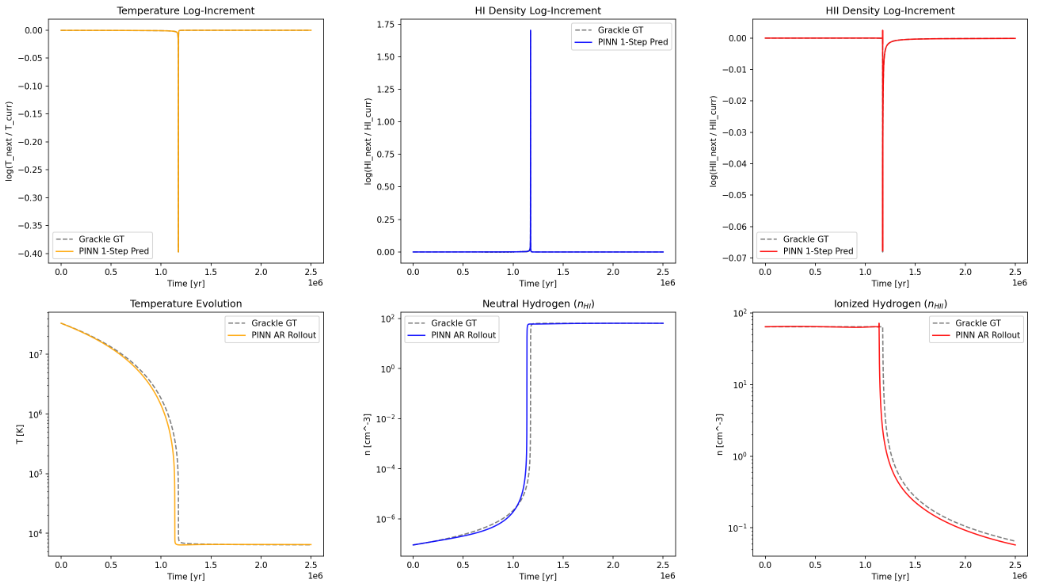
\includegraphics[scale=0.55]{images/GoodPreds-ModelA.png}
    \caption{Good predictions of Model A on a given Family 3 trajectory. Top: log-increment predictions. Bottom: linearised predictions.}
    \label{fig:GoodPreds-ModelA}
\end{figure}

\begin{figure}[h!]
    \centering
    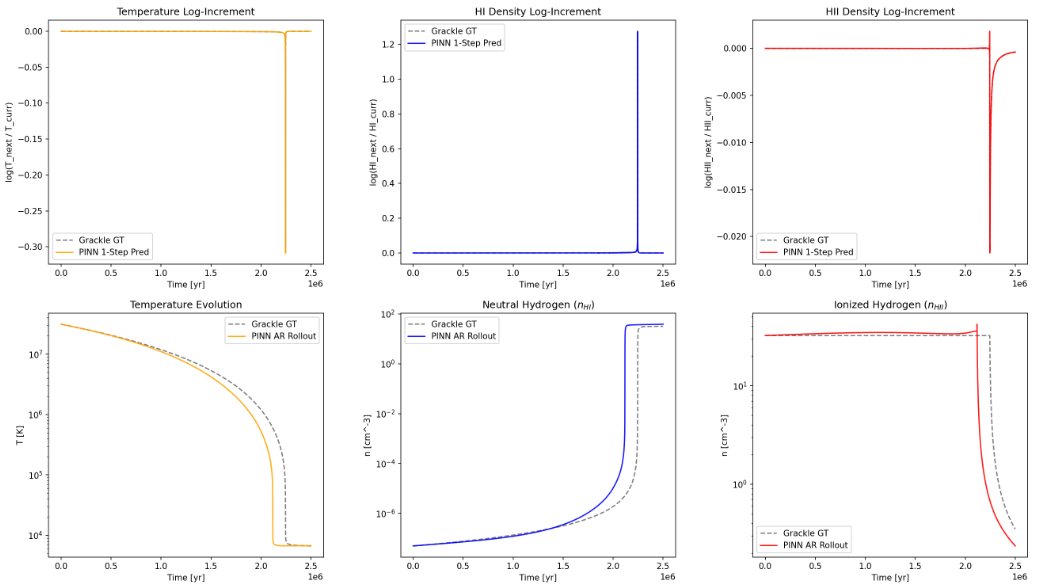
\includegraphics[scale=0.55]{images/GoodPreds-2-ModelA.png}
    \caption{Slightly degraded predictions of Model A on another Family 3 trajectory. Top: log-increment predictions. Bottom: linearised predictions.}
    \label{fig:GoodPreds2-ModelA}
\end{figure}

\begin{figure}[h!]
    \centering
    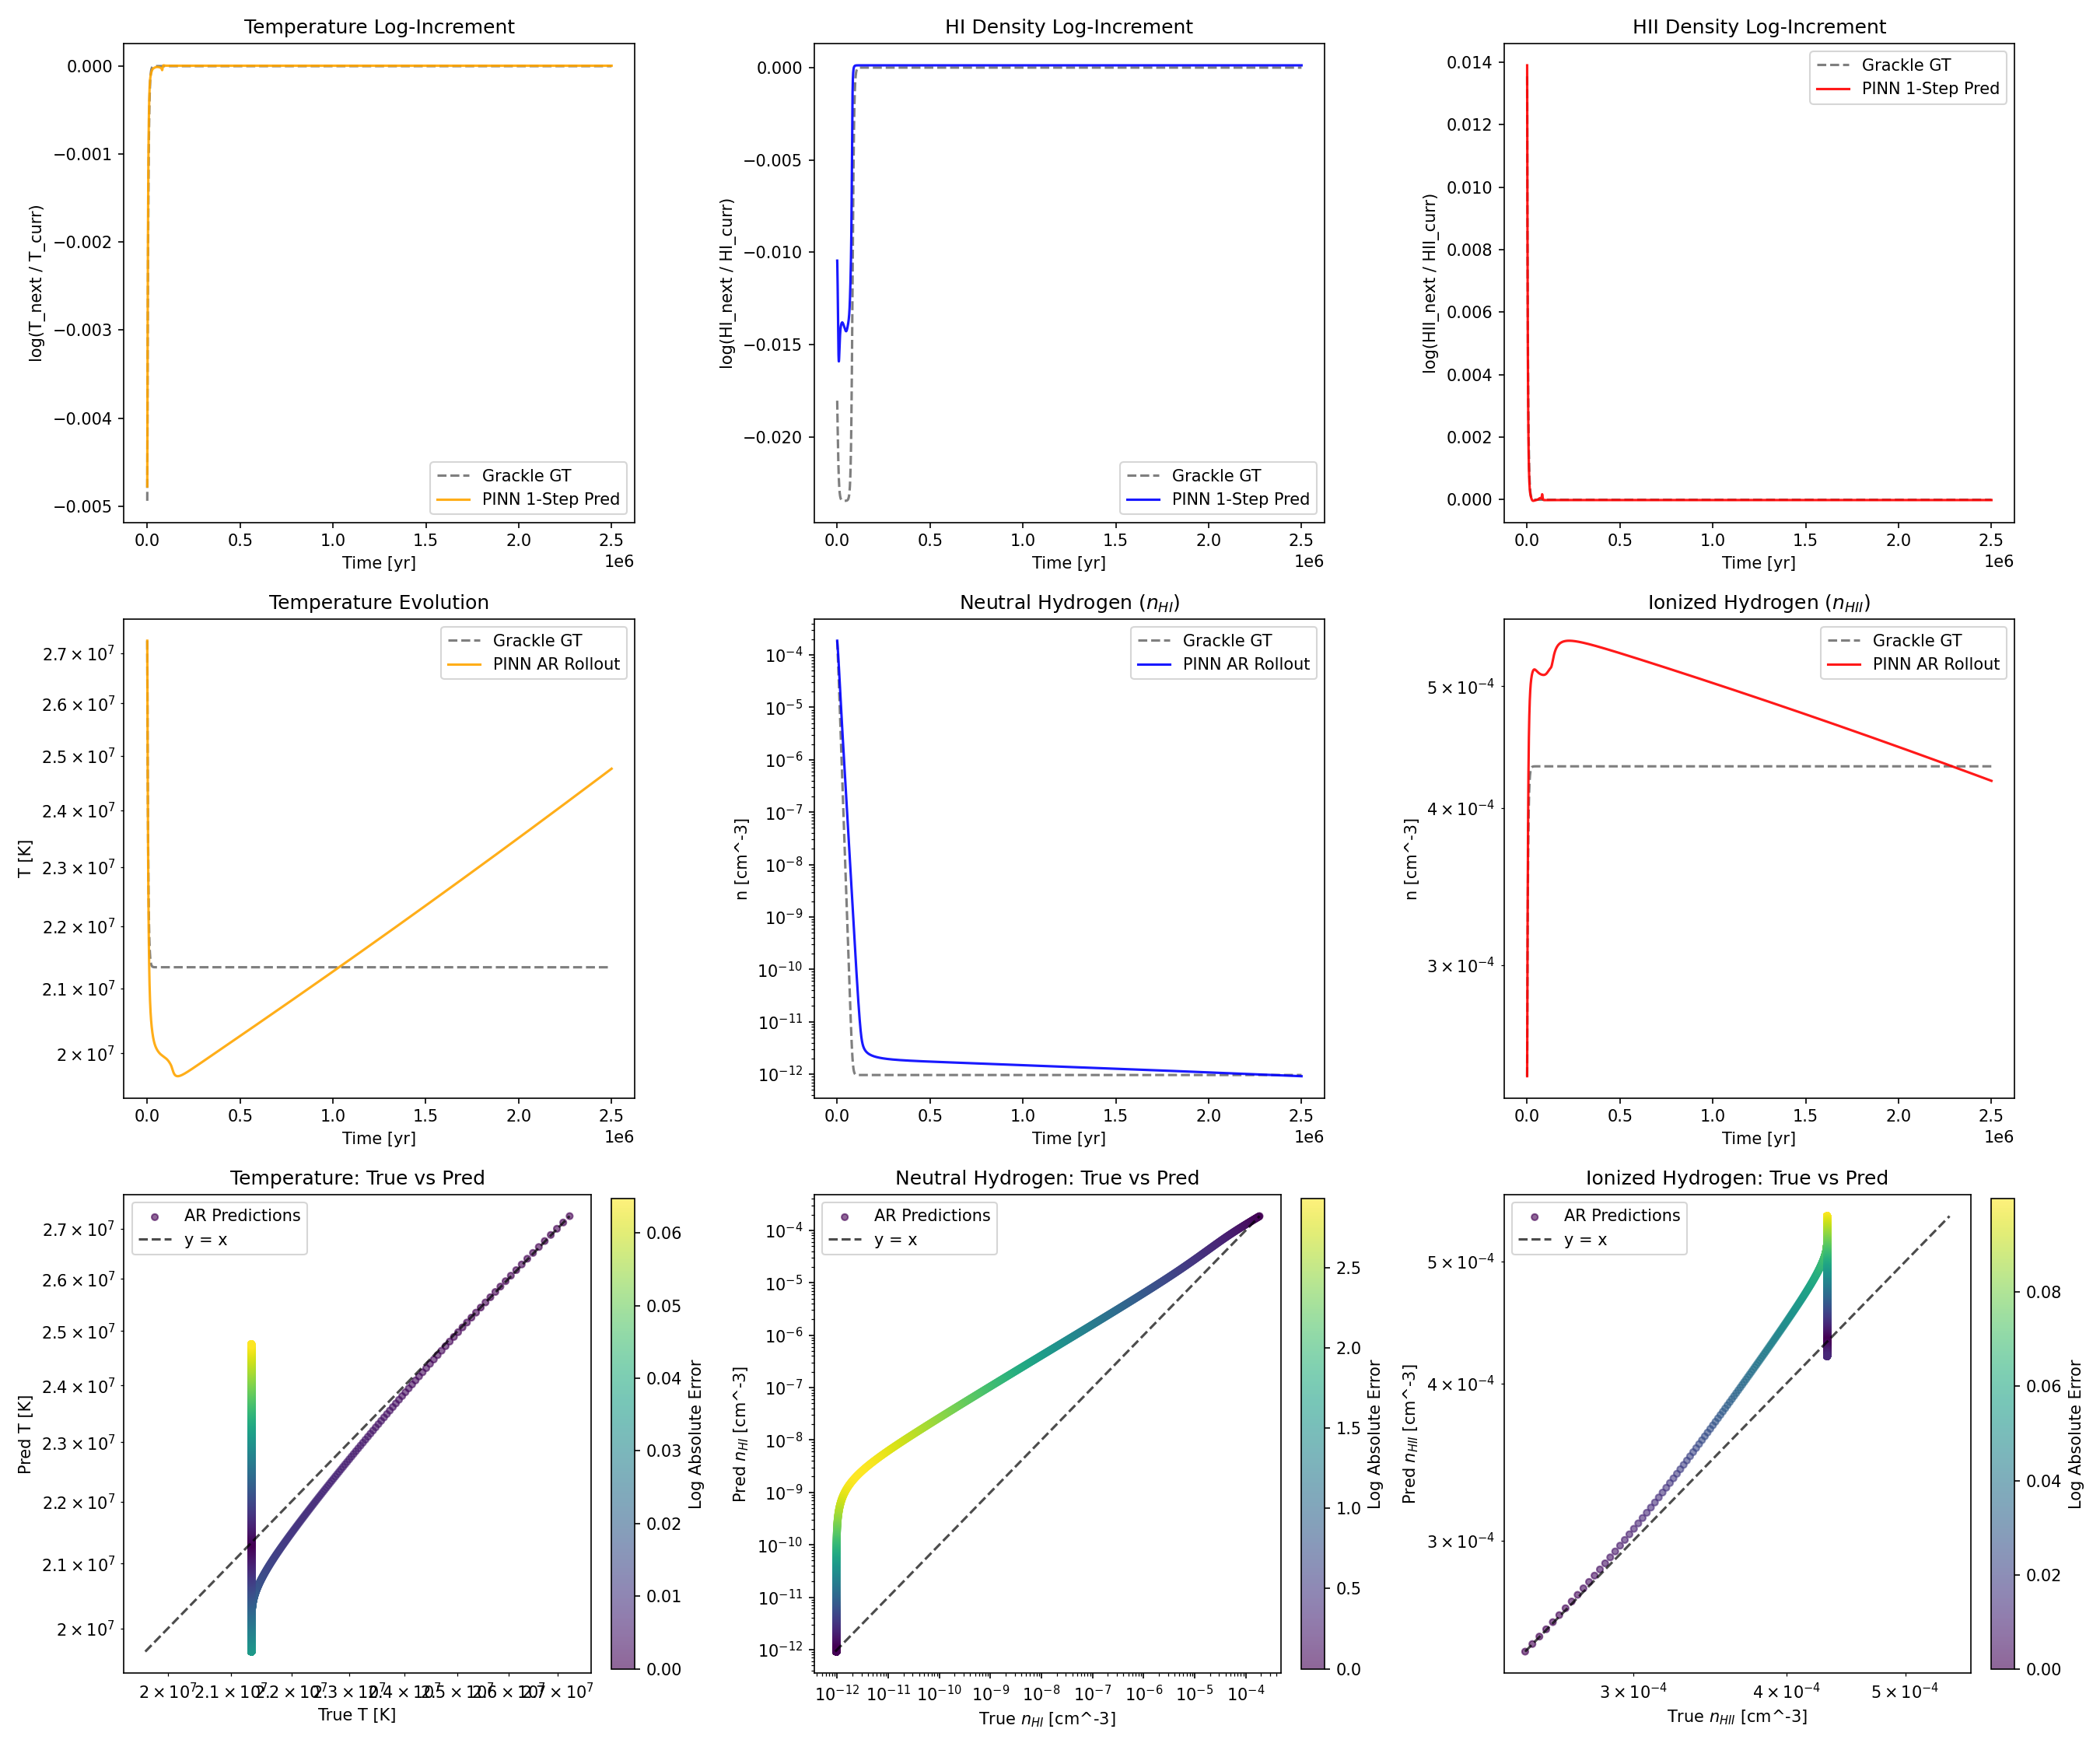
\includegraphics[scale=0.3]{images/fam0.png}
    \caption{Widely degraded predictions of Model A on a Family 0 trajectory. Top: log-increment predictions. Middle: linearised predictions. Bottom: x-y plot of true vs linearised predictions.}
    \label{fig:fam0-modelA}
\end{figure}

\begin{figure}[h!]
    \centering
    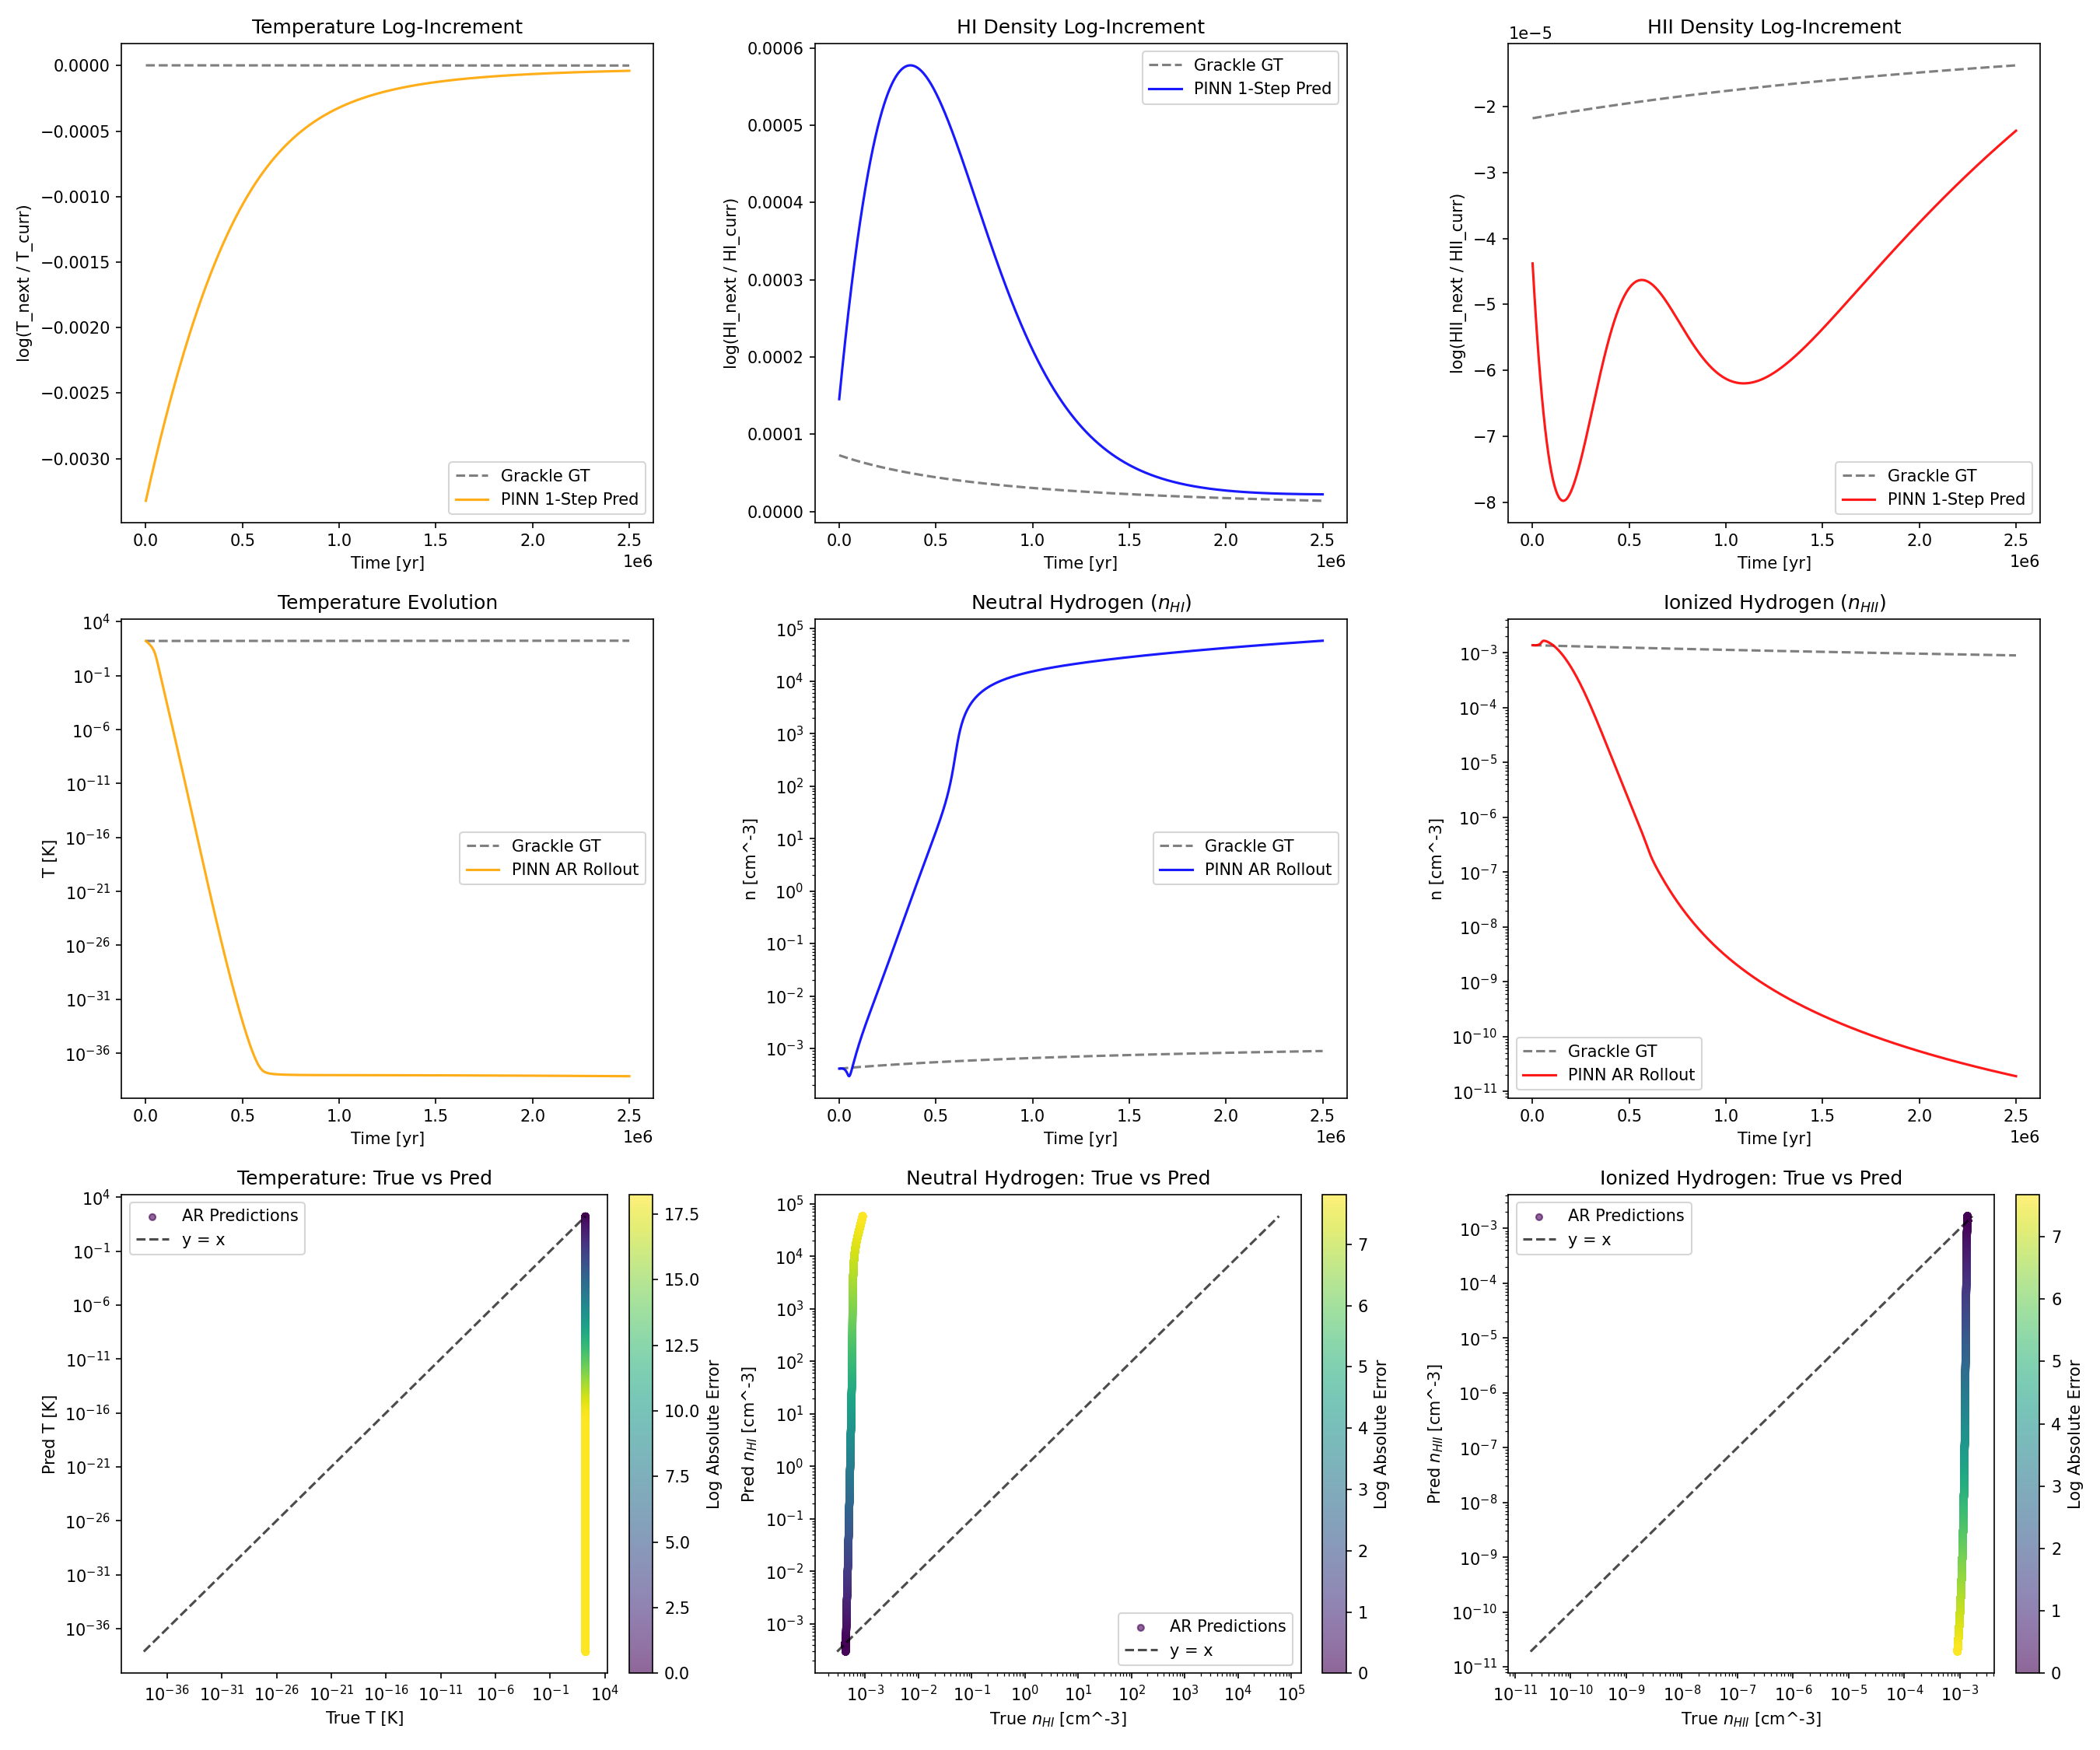
\includegraphics[scale=0.3]{images/fam1.png}
    \caption{Widely degraded predictions of Model A on a Family 1 trajectory. Top: log-increment predictions. Middle: linearised predictions. Bottom: x-y plot of true vs linearised predictions.}
    \label{fig:fam1-modelA}
\end{figure}

\begin{figure}[h!]
    \centering
    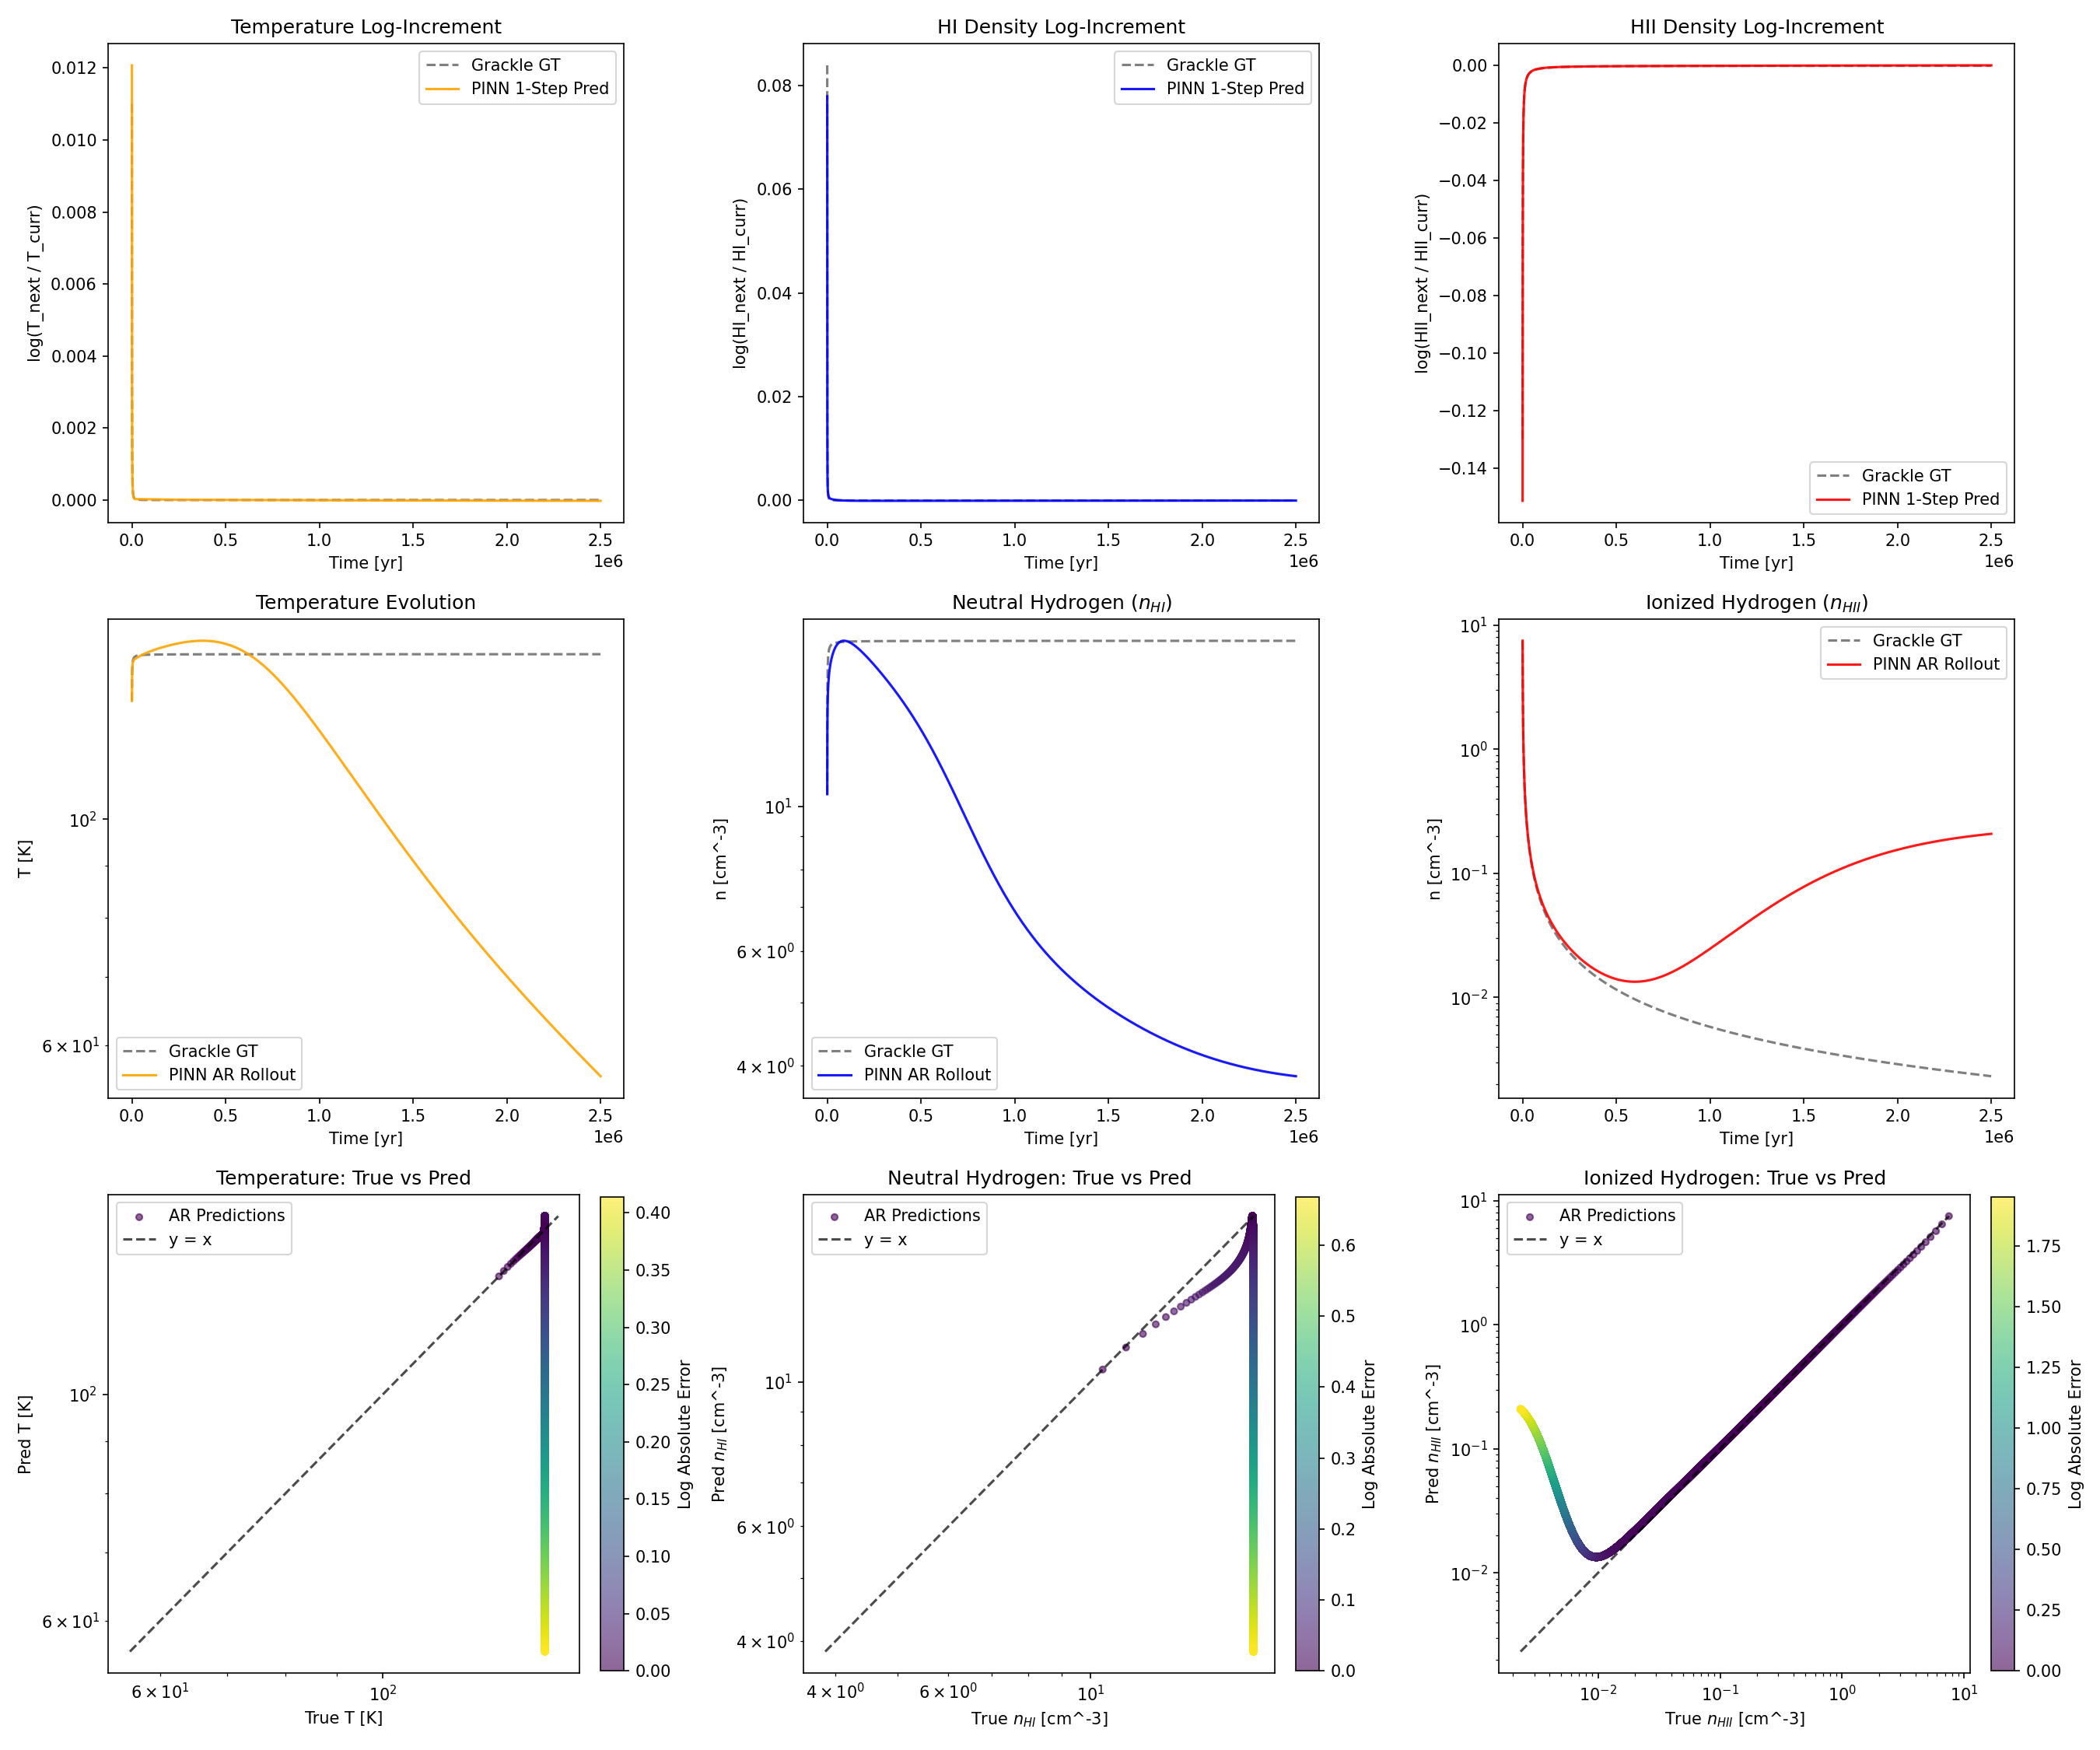
\includegraphics[scale=0.3]{images/fam2.png}
    \caption{Widely degraded predictions of Model A on a Family 2 trajectory. Top: log-increment predictions. Middle: linearised predictions. Bottom: x-y plot of true vs linearised predictions.}
    \label{fig:fam2-modelA}
\end{figure}



\end{document}